\section{Discussion}\label{sec:analysis}
% \subsection{Training setup}\label{sub:setup}
% Why we used expert choice, specific models etc.

% \subsection{Autoregressive Expert Choice}
% Other interesting results: expert choice for autoregressive models (group size matters); expert choice evaluated as token choice; results for varying expansion rate. Our Granular MoE, in contrast to regular Expert Choice can be used on each layer, bringing in consistently to the architecture.

% \subsection{Fine-Tuning Expert Choice as Token Choice}
% In our experiments we explored the impact of routing strategies on model performance. Initially employing standard expert-choice routing, where each expert chooses some number of tokens from each position in sequence from fraction of batches, independently for each position in sequence, we observed a significant decrease in model performance when transitioning to token-choice routing, where each token determines the fraction of experts it attends to, while keeping all weights unchanged.

% To address the performance decline in token-choice routing, we fine-tuned the model trained with expert-choice routing to token-choice routing without introducing additional balancing loss, a typical component countering routing imbalance \cite{shazeer2017outrageously, fedus2022switch}. Remarkably, the fine-tuned model, rapidly rebounded to a perplexity level comparable to that of expert choice, highlighting the adaptability of the MoE architecture.

% These results hold promise, particularly since evaluating as an expert-choice requires a large batch, a constraint that is not universally applicable. In contrast, token-choice routing proves to be batch-size independent and, given its comparable effectiveness to expert choice, emerges as a superior alternative at inference.
% \sj{Include, somewhere, "There is a need to include transfer costs, and not only FLOPs, in Scaling Laws, especially with MoE. While this is extremely hardware dependent, and still number of FLOPs.}
% \jk{dodać jakiś wykresik że nasze predykcje korespondują z czasem. To widać np. na medium z }
% \jk{dodaję Future Work do tytułu, można to usunąć. Ale wydaje mi się że w dużym stopniu mamy tu Future Work}


\paragraph{Extreme Granularity.}
In Section \ref{sec:scaling_laws}, we argue that model performance improves with increasing granularity. This postulate largely aligns with the empirical findings of our study. Nonetheless, at exceedingly high granularity levels, such as $G=64$ in models characterized by $\dmodel=256$  and $E=64$, there is an observable decline in performance. This phenomenon is particularly evident in scenarios where the number of parameters in the routing mechanism exceeds active parameters in actual experts. Additionally, as described in Section \ref{sec:scaling_app}, the utility of such high granularity is predominantly restricted to models of substantial size. In alignment with the principles outlined by \cite{hoffmann2022training}, this research focuses more on findings that can be broadly applied rather than delving into the specific details of these corner-case situations. However, it is hypothesized that the efficiency of models with significantly high granularity could be potentially enhanced through careful expert initialization or modifications to the routing algorithm. These ideas are set aside to be investigated in future studies.

\paragraph{Varying Expansion Rate.}
In this study, due to computational resources constraint, we focus on $E=64,$ as recommended by \cite{clark2022unified}. This value of $E$ was also used for the largest models in other works \citep{du2022glam, zhou2022mixtureofexperts} and the best-performing configuration in \cite{fedus2022switch}. Nonetheless, we acknowledge the importance of considering different expansion rates, as different levels of $E$ may be chosen based on factors like the target size of the model in memory. Therefore, in Appendix~\ref{app:exp_rate}, we present the results of the study for $E=16$ and show that the main findings of this work are still valid in such cases. 
%The number of experiments needed to consider various values of expansion rate has made it practically infeasible for us, as we already model dataset size and granularity. 
%\janek{to jedno nastepne zdanie bym przerzucil juz do tego appenixu} In particular, higher granularity is more optimal when increasing the compute budget. We also observe that with $E=16$ MoE models always outperform dense Transformers, and that the gap widens with scale.

\paragraph{Including $E$ in the formula.} Another possible advancement would be to unify all of the factors $N, D, G$ and $E$ in one formula. While this would open the possibility of studying the relationships between coefficients in more detail, it would also be hard to practically recommend the optimal configuration in such a scenario using only FLOPs. This is because larger values of $E$ typically lead to better performance but also incur additional memory requirements. Therefore, the choice of expansion rate may be heavily dependent on the available hardware configuration. We leave a detailed study of these factors for future work.

% (tutaj opisujemy, że tak naprawde extreme granularity się wygina i nie wiemy czemu, ale jest to zawsze dalekie od optimum a nasze scaling laws opisuja tak jak wszystkie laws modele niezdegenerowane. Może to wynikać z tego że w pewnym poziomie liczba parametrów w routingu jest większa niż w FF i napewno nie chcemy do takiej sytuacji doprowadzać albo od potencjalnie innej inicjalizacji)

\paragraph{Modeling the cost of granularity.}
It is important to note that the exact estimation of the training cost of MoE models is dependent on the training setup, hardware, and implementation. Specifically, increasing G can lead to higher transfer costs, depending on the adopted model of distributed training. Therefore, the precise selection of hyperparameters should be made considering these factors. In this work, we model the cost of operations using FLOPs, which is common in the Scaling Laws literature \citep{kaplan2020scaling, hoffmann2022training, frantar2023scaling}. Additionally, we would like to note that in our setup, we observe significant gains of fine-grained MoE measured as wall-clock time needed to achieve given perplexity (see Fig. \ref{fig:valid_wall} (b) for an example).  

% \begin{figure}[ht!]
% \centering
% 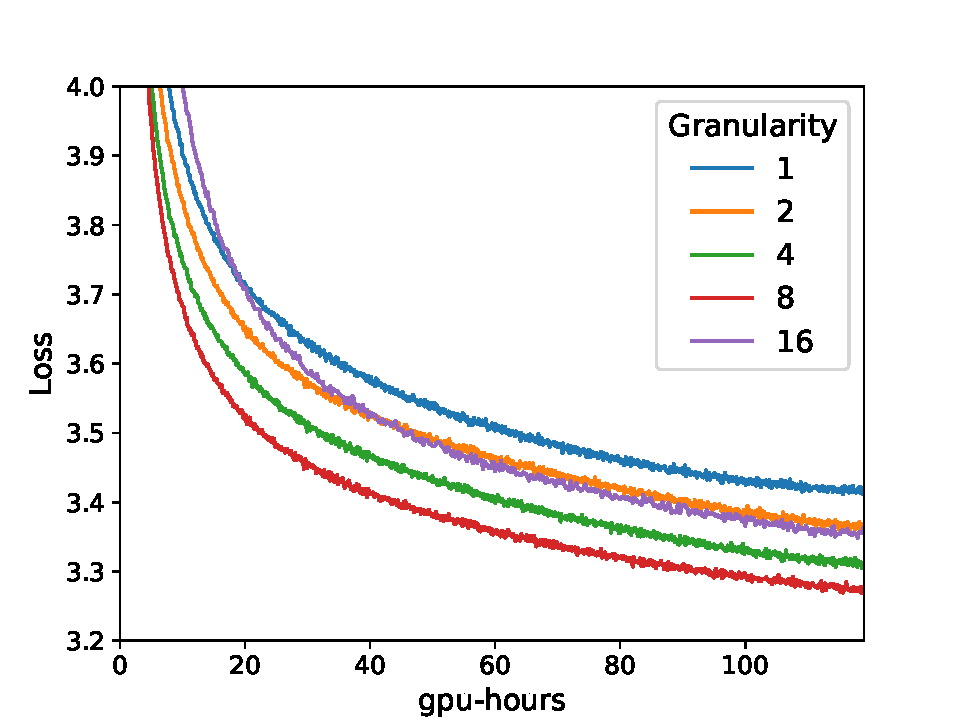
\includegraphics[width=0.6\textwidth]{figures/time.pdf}
% \caption{Training loss curves for model with $N=64 \times 7M$, $D=66B$ tokens, measured on NVIDIA A100 GPU. We can see that the model
% with $G=8$ achieves the best performance.}
% \label{fig:time}
% \end{figure}

% \jk{Jak zdążymy, dla uczciwości można coś dodać że te scaling laws moga być zależne od dokładnego setupu (typu tokenizer, dataset, itp. }

% \subsection{Larger Scale}
% In this study, we derive our conclusions based on over 100 experiments, spanning various parameters for dense and MoE models. While we are able to match the model sizes considered by \cite{kaplan2020scaling}, our compute capabilities are...
% W punktach, co tu ma być:
% 1. O ile rozważane przez nas wielkości modeli są porównywalne do tych używanych w [kaplan], nasze ograniczenia budżetu obliczeniowego są istotniejsze niż w przypadku 
% \jk{Tutaj jakaś obrona, dlaczego mamy takie wielkości modeli. Ze w sumie nasze modele są całkiem spore (total params), i że Kaplan też miał podobne. No ale że jakbyśmy mieli więcej compute, to byśmy dokładniej skalibrowali nasze wyniki. I że mimo wszystko nasze główne wnioski pozostają w mocy.}
% \jk{coś że nasze wyliczenia mogłyby być dokładniejsze}
